
\begin{figure}
    \centering
    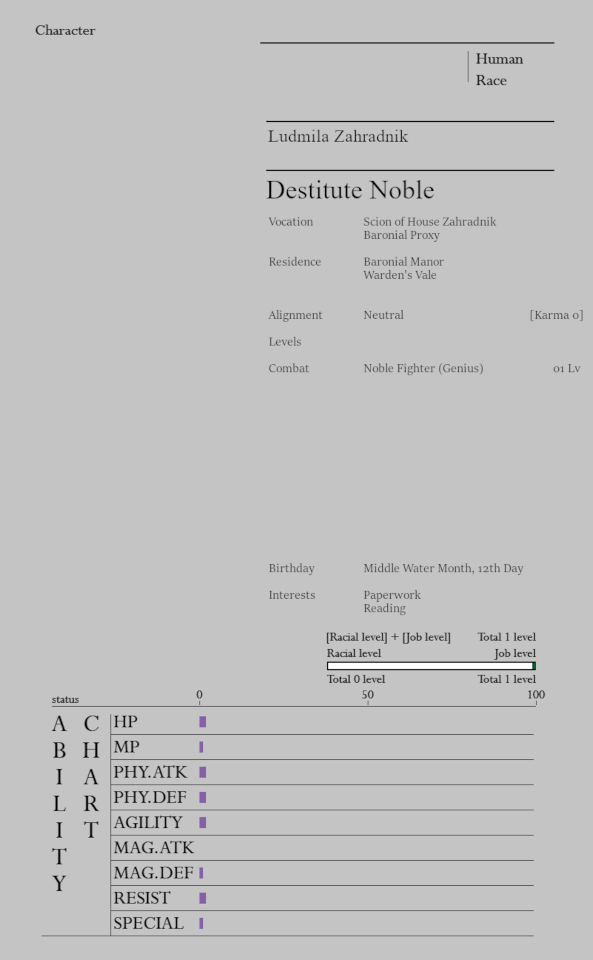
\includegraphics[width=0.9\linewidth]{images/9rood84.png}
    \caption*{Ludmila Zahradnik Character Sheet, Act 1 Chap 1}
\end{figure}

\section*{Class Highlight: Noble Fighter}
From the brash tales of bawdy musicians in seedy taverns to the sweeping epics of eloquent minstrels in the highest imperial courts, the annals of history sing the tales of storied nobles who wield both pen and sword with equal proficiency. They rule wisely from their high courts and lead grand armies on the field; performing legendary acts of valour in service of king and country.

The Noble Fighter is a living manifestation of this history, frequently appearing as nations rise and necessity drives their leaders to become directly involved in the security and direction of its nascent territories. As a variant of the Fighter class, they forego the general freedom that is usually associated with a Fighter’s non-combat skillset, instead specializing in the disciplines that revolve around leadership and administration while retaining the Fighter class’ personal martial prowess.

As feudal societies achieve a greater measure of security, stability and prosperity, Noble Fighters become increasingly scarce. However, while aristocrats of pure civilian focus become more prolific as nations develop to maturity, Noble Fighters may still be found where duty or necessity demands their presence. Scions with no realistic prospect of inheritance may seek a martial path, aspiring to serve as a member of a noble retinue, professional army or knightly order while retaining their aristocratic ties. Regions with strong military traditions or fiefs wherein noble houses are expected to guard the realm against foreign threats will also tend to produce Noble Fighters from within the ranks of their ruling elite.

Contrary to the flowery image painted by romantic tales, Noble Fighters are not necessarily benevolent. They are exemplars of militant aristocracy, striving to uphold a well-rounded portfolio of effective governance, leadership and martial proficiency expressed through actions that may range throughout the moral spectrum.

\chapter{Ludmila Zahradnik}

The sound of a distant bell arose from below, its sharp toll rolling up from the riverbank and washing over the buildings of the village on the hill. They were of simple construction: affairs of sod and stone visibly overgrown by creeping vines and layers of thick, green moss. Little but their humble faces peeked out from the weathered terraces cut deep into the rocky slopes by generations long gone; such was their appearance that even a lowly farmhand from the fertile lowlands might have scoffed.

 

The inhabitants of the village were well accustomed to their homes, however, and would have politely ignored such derision as they were generally satisfied with their current arrangement. The hill stood near the head of a long valley with high slopes that were nearly impassable by Human measure. A large river ran its course around the hill and northwards through to the narrow gorge beyond while a vast and marshy floodplain filled most of the valley floor. Approaches by land were treacherous in addition to being highly vulnerable and difficult to conceal. Even lacking the walls one might find around larger towns and cities, the layered terraces of the village stood as effective ramparts against all but the most determined of savage and lawless raiders.

 

A more militant mind might have noted all these qualities and inferred that the settlement was built with defence in mind; they would have been exactly right. Warden’s Vale lay in the shadow of the Southern Border Ranges, at the far southwestern reaches of the Duchy of E-Rantel. It was the seat of House Zahradnik, one of the noble lineages that guarded the frontiers of the Kingdom of Re-Estize. Beyond the Vale lay an increasingly vast wilderness: populated by Demihuman tribes, monsters and worse.

 

It was an island of relative safety in a land otherwise hostile to Human habitation. The homes nestled in the hill were well-insulated and offered warmth in the highlands where the deep winter months were often visited by biting cold and blankets of snow. Through generations of stubborn vigilance, the hardy frontiersmen had carved out a permanent presence that was now left mostly uncontested by their neighbors – simply put, they had proven that they were more trouble than they were worth.

 

Roughly halfway up the hill, a single dwelling stood distinct from the rest. The lord’s manor possessed the same simple construction as the other homes built around it, save for a large extension constructed out of well-worn wood which jutted out conspicuously onto the widened terrace that it was built on. This space served as the main hall of the manor: the office of the Barony.

 

Its thin wooden walls did very little to dampen the sound coming from below and the hall was soon filled with the bell’s lonely peal where only the scratching of quill on parchment could be heard just moments before. The slim hand which was guiding the quill rose at the sound, arresting the instrument’s flowing dance and raising it over its simple stage as dark ink dried below. After several moments of silence, the bell repeated its urgent call for attention and the grey goose quill was carefully set aside.

 

Ludmila raised her head with a slight furrow on her brow, turning to look out of the window that spilled light over the well-worn wooden desk. The bell was used for a handful of purposes: calling the faithful to religious services, an alarm for fire and flood, rallying the villagers against external threats and for communication along the river. Though the distinct pattern was recognizable as the last of these, she still scanned the immediate surroundings in the yard and village before directing her vision further beyond.

 

It was a clear afternoon – rare for late winter on the edge of the border ranges. The sun was well past its zenith, approaching the western ridge that overlooked the valley wherein the settlement lay; casting long shadows over its soggy flats. In the distance where the river disappeared into the gorge to the north, a billowing sail caught the light of the afternoon sun; immediately drawing the attention of any observer that happened to look in its direction.

 

It was a familiar sight, yet entirely unexpected. There were only two ports on the river and the single vessel that currently operated between them was the one owned and operated by their own village. As the winds blowing southwards up the valley coaxed the ship upstream, the bell’s call remained unanswered; each pause and repetition only served to punctuate a growing sense of unease.

 

Rising from her seat, she cleaned her ink-stained fingers on a damp rag tied to a corner of the desk before picking up the simple leather-bound ledger she had been working out of. She blew lightly on its open pages in an effort to help the ink dry as she made her way to a cabinet at the back of the hall, the keyring on her belt jingling as she padded across the stone floor. After carefully putting away her work and securing the lock on the cabinet, she snatched a plain, unembroidered shawl that was draped over a chair in the dining area. Ludmila retraced her way back through the hall towards the manor entrance, her steps slowing slightly as she focused on wrapping the cloth securely about her head and shoulders.

 

The frigid air carried by the winds of winter greeted her as she opened the door and made her way onto the narrow lane leading from her home. Though the layered fabrics of her dress blocked out most of the cold, wisps of air still occasionally seeped through to nibble at her skin. With the ship steadily making its way up the river to the pier, she paid it little mind. It had barely been a fortnight since the vessel had last left; bearing away Baron Zahradnik and many of the men of the village: a levy raised to defend the Kingdom of Re-Estize against an uncharacteristically late challenge presented this year by the Baharuth Empire.

 

In truth, it had long since become an annual occurrence so there was very little fuss surrounding it. By all accounts, the two sides would meet with their armies on the cursed fields of the Katze Plains and skirmish halfheartedly before withdrawing. This would continue over the course of several weeks before honour was satisfied and both sides struck their camps to return home. The Empire always seemed focused on conserving the fighting strength of its Legions and refused to commit to a pitched battle. Similarly, the forces of the Kingdom had no reason to go on the offence – and no reason to deplete the levies formed out of their everyday pool of labour – so casualties were relatively light for both sides. Most years, the seasoned men of the frontier village would return with barely a scratch.

 

The great houses of Re-Estize would use the campaign season to posture and jockey for prestige and influence, but to the nobles of Re-Estize who did not attend the Royal Court, it was generally an annoyance that drew manpower away during the harvest season while disrupting the productivity and flow of goods throughout the realm. With the call to arms being so late this year, however, the fields had long since been cleared and it was received as an almost welcome distraction for the men. They would otherwise likely be driving their families crazy while being cooped up around their homes as the cold, short winter days wore on. Still, they were not expected back for at least a full month after their departure, perhaps even two.

 

Ludmila made her way past the cozy abodes of the villagers and down the rugged lane towards the riverbank. The main passage that wound through the village was laid with uneven stones of various sizes, hauled up from the shore. It was something that had happened over time as the villagers acted to make the often muddy slope of the trail easier to scale, resulting in a makeshift cobblestone path. Wooden planks in various stages of wear served as simple steps over its steepest portions.

 

She mulled over the possibilities that could result in an early return, but couldn’t come up with anything that made any real sense given what she knew. Many of the villagers had come out of their homes by now, curiously looking out towards the approaching vessel. In this isolated valley on the Kingdom’s southern border, life was mostly slow and uneventful so this sort of occurrence was what amounted to a major event. Some followed after her as she passed by while others simply stood about gathered with their neighbors in small groups as they spectated from a distance.

 

By the time she reached the base of the hill, there was a modest crowd of people already waiting for the boat’s arrival. Nearly all were women related to the men that had been drafted as part of the levy and most looked on anxiously with the same confused atmosphere that had followed Ludmila on her way down the terraced path. Though they were mostly dressed in a similar fashion to herself, all made room as she approached, nodding respectfully in silent recognition.

 

At the spot along the shore where the pier extended out into the river there was a large brass bell that hung on its wooden frame; well worn through countless years of service but still carefully maintained. It was from here that the periodic signalling that had urged her to step away from her work and investigate had issued forth. A girl several years younger than her stood under it with her hand gripping the sally: she recognized her as the younger sister of one of the men who regularly served as part of the fief’s patrols – the girl had taken up sentry duty in her brother’s absence.

 

Ludmila stood a short distance away as the girl repeated the signal. There was a long pause as the operator waited once again for a response...

 

Nothing.

 

The furrow on Ludmila’s brow appeared once again – if one of her brothers had been there to look at her face, he would have probably teased her about getting wrinkles before twenty. However, there were few who knew how to navigate ships on the river and all of them should have known how to communicate along it. This lack of a response filled her with disquieting notions: images of a ship concealing bandits or Demihuman raiders began to form in her mind. Though she had never heard of such a thing happening before in this area of Re-Estize, she was at a complete loss as to what was going on and her imagination began to formulate fantastical scenarios with the unknowns presented.

 

After failing to solicit a response from the approaching vessel yet again, the girl looked to Ludmila. The worried expression on her face seemed to ask whether she had improperly sounded, since the approaching vessel had never answered. Ludmila could only smile slightly while placing a hand over the girl’s shoulder reassuringly as she gently guided her away from the edge of the water with the ship looming ever closer.

 

By now, she could clearly make out the details and the murmur that rose from the common folk around her mirrored her own thoughts. The ship was now irrefutably recognizable as the one that belonged to the village. It was a nameless craft of shallow draught that had seen decades of use: its billowing sail and wooden construction were a patchwork of repairs and improvements that marked the tale of its long service to the Barony.

 

Aside from a man working the rudder to guide the vessel upriver, no one else could be seen. When the ship had departed earlier in the winter, it carried just over three dozen passengers – which was around three quarters of the seasoned men available. They were all in good spirits and sat tall amongst the equipment and supplies that would follow them to war. Their distinct absence on the ship created a collective sense of unease that steadily grew over the gathering on the shore.

 

At Ludmila’s direction, two stout, middle-aged housewives tied up their layered skirts and waded into the shallows to draw the vessel in as it neared the pier. It was only when it came close enough for them to peer over and inside that she saw there were more people on board. Four other men were inside: two were sitting curled up with their arms around their knees while the other two lay sprawled on the bottom of the bare wooden deck like puppets whose strings had been cut. All seemed to be awake – or at least their eyes were open – but they did not appear to be aware of their surroundings.

 

The strange scene stretched on, with the onlookers unsure what to make of it. Finally, a woman leaned forward, extending a tentative hand towards the nearest person curled up in the boat. She was the mother of the young man: mustering the courage to reach out to her child...but before she could touch him, a rogue wave caused the boat to bump up against the pier with a slosh and a thump.

 

He started suddenly, jumping up while shouting incoherently, clawing at the edge of the boat for a handhold before scrabbling onto the damp earth of the pier. Ludmila and several others, startled at his sudden movement, collectively stepped back out of caution at the irregular behaviour. Not a moment later, he began moving again...but rather than rising to his feet, he was hunched over, his fingers nearly brushing the ground. She briefly made eye contact with him before he lunged forward, shoving her out of the way. Ludmila's arms flailed out as she staggered and struggled to maintain her balance until hands reached out to steady her from behind.

 

By the time she turned to angrily call out to the man, he had already made his way partway up the hill, scaling the slope on all fours on a mad crawl towards his home. His worried mother followed after him, though nowhere near fast enough to keep up with his frenzied pace. Ludmila's anger subsided as quickly as it had risen upon witnessing this bizarre scene, recalling the man's gaze just a moment earlier: rather than a person, his sunken, bloodshot eyes had looked at her as if she was some obstacle, like a branch in an overgrown trail to be pushed aside.

 

Expelling a deep breath, Ludmila tamped down on her emotions as she turned back to the ship, hoping to make sense of the strange event unfolding before her. The girl who had been signaling with the bell had dropped down to the deck of the ship and was trying to rouse the second man curled up in the boat – her brother. The two other men that lay catatonic on the deck had not stirred even after the disturbance, but the man working the rudder had vanished during the commotion. Ludmila scanned the vessel from bow to stern: there was no sign of any belongings being brought along, neither was there any recent damage that suggested that they had been attacked. The undisturbed emptiness of the ship led her to the conclusion that they had departed in a hurry, with no time to load fresh supplies or even wait for their fellow villagers.

 

As time wore on, the small crowd watching from the shore dispersed, carrying the uneasy atmosphere with them. Ludmila gave instructions for the two men on the deck to be carried out and tended to while a few villagers still remained, then stepped down onto the boat beside the girl and her brother. With her sister's worried urging, the man's previously empty gaze had turned somewhat lucid again and Ludmila reached out to help him to his feet.

 

As she and the man’s sister guided his unsteady steps off of the pier and onto the path into the village, Ludmila decided to try and find out what was going on.

 

“Milivoj, what happened? Where is everyone else? Where is the Baron?”

 

With the guardsman in his clearly shaken state, she kept her phrases as clear and simple as possible.

 

If he had heard her, he gave no sign of it. The soles of his boots scraped against the wooden planks laid on the path between the pier and the village proper as he shuffled forward. The man's still-bleak gaze remained downcast, even after she released his arm. A part of her wanted to shake him to get his attention but he had such a frail, unstable appearance that she thought he would fly apart mentally like the other man if she did.

 

Before long, they had reached the home of Milivoj and his sister. After taking her brother inside, the young girl curtseyed awkwardly to Ludmila before quietly closing the door. Left standing alone on the path, she turned around to look out over the village. The evening sun had dipped below the ridge of the valley, shrouding the hill in gloom.

 

Normally, people would be finishing their day’s work around this time, lingering outside to socialize and relax. Witnessing the disturbing scene that evening, however, everyone had withdrawn into their homes instead. Ludmila let out a sigh as she started walking back to the manor. Life out in the rural regions of the Kingdom revolved around the daytime hours and she would probably not be able to see anyone until the morning. Well, not that anyone seemed to be in the mood or condition to speak.

 

The freezing chill of the evening made the fading indigo sky seem even more crisp than usual. Turning her head upwards, Ludmila watched silently as the brightest stars made their appearance overhead. The tension that had suddenly built up over the course of less than an hour slowly seeped away from her as she took in the sight, yet the unsettling feeling deep in the pit of her stomach remained. Feeling drained in both mind and body, she walked back up the path to the manor with disquieting fears whispering from the dark corners of her mind. Slowly making her way up through the terraces of the village, she decided that it would be best to retire early for the night. Hopefully the men that had returned would be well enough the following morning to tell her of what had happened at Katze.